\begin{frame}{Data Pre-Processing}

    \begin{minipage}{0.5\textwidth}
          Our data set presented to be ready to use as:
        \begin{itemize}
            \item There were no missing values
            \item There were no apparent measurement errors
            \item There were many outliers but they did not represent any errors and were, in all likelihood, the exact object of our analysis
        \end{itemize}
    \end{minipage}%
    \begin{minipage}{0.5\textwidth}
        \begin{figure}
            \centering
            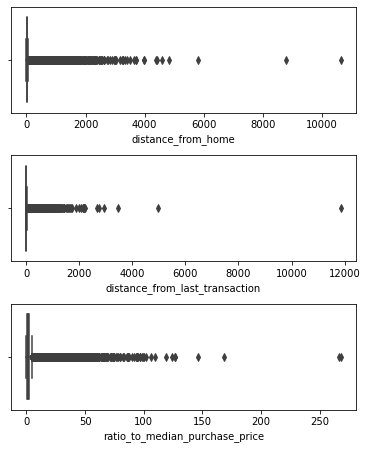
\includegraphics[width=0.65\textwidth]{images/boxplots.png}
            \caption{Boxplots}
            \label{fig:my_label}
        \end{figure}
    \end{minipage}

\end{frame}

\begin{frame}{Exploratory Data Analysis}

    \begin{minipage}{0.5\textwidth}
        Performing an \textbf{Exploratory Data Analysis} we concluded that:
        \begin{itemize}
            \item As previously mentioned, our data set was moderately imbalanced (classification label is binary and 8.7\% of the entries represent fraudulent transactions).
            \item Many of the features had little relation with the label feature, as their values did not vary much between the two label classes and their correlation was very low. 
        \end{itemize}
    \end{minipage}%
    \begin{minipage}{0.5\textwidth}
        \begin{figure}
            \centering
            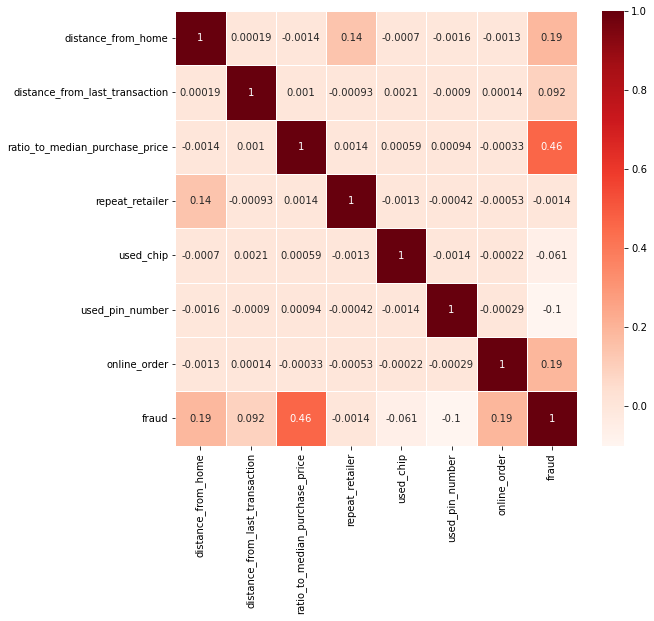
\includegraphics[width=0.85\textwidth]{images/output.png}
            \caption{Correlation Matrix}
            \label{fig:my_label}
        \end{figure}
    \end{minipage}

    
    
    
\end{frame}